\documentclass{article}
\usepackage{graphicx}
\title{Five-lead genus-2 collector: operation-cost evidence}
\author{Crypto research evidence package}
\date{2026-10-19}
\begin{document}
\maketitle
\section*{Scope and method}
This report summarizes the frozen two-choice genus-2 relation-collector cohort in the five-lead study. It contains 21 exact-order curves, seven source-order sizes (16 through 40 bits), 60 paired one-target workloads per curve, and 1,260 targets in total. All six arms across the cohort are source-verified and independently replayed (6,300 records); see the study replay-audit summary and packed session archive.

The graph uses deterministic operation-count costs from the frozen price grid at $M+0.5S+10I$, plus a $0.1M$ charge per declared native logical operation. Ratios are sums of paired costs, not averages of curve ratios. Ratios above 1 mean the two-choice candidate incurred higher operation cost. Each size point pools 180 paired targets. The pooled reference uses all 1,260 targets.

\section*{Observed ratios}
\begin{center}
\begin{tabular}{r|r|r|r}
Source order bits & Paired targets & Choice2 / incumbent & Choice2 / rho-neg \\
\hline
16 & 180 & 0.943697 & 3.812897 \\
20 & 180 & 0.972590 & 3.824903 \\
24 & 180 & 0.981876 & 4.229300 \\
28 & 180 & 0.988278 & 4.373698 \\
32 & 180 & 1.018553 & 4.366459 \\
36 & 180 & 1.027152 & 4.694925 \\
40 & 180 & 0.993748 & 4.444705 \\
\hline
Pooled & 1,260 & 1.000857 & 4.483247 \\
\end{tabular}
\end{center}

\begin{figure}[ht]
\centering
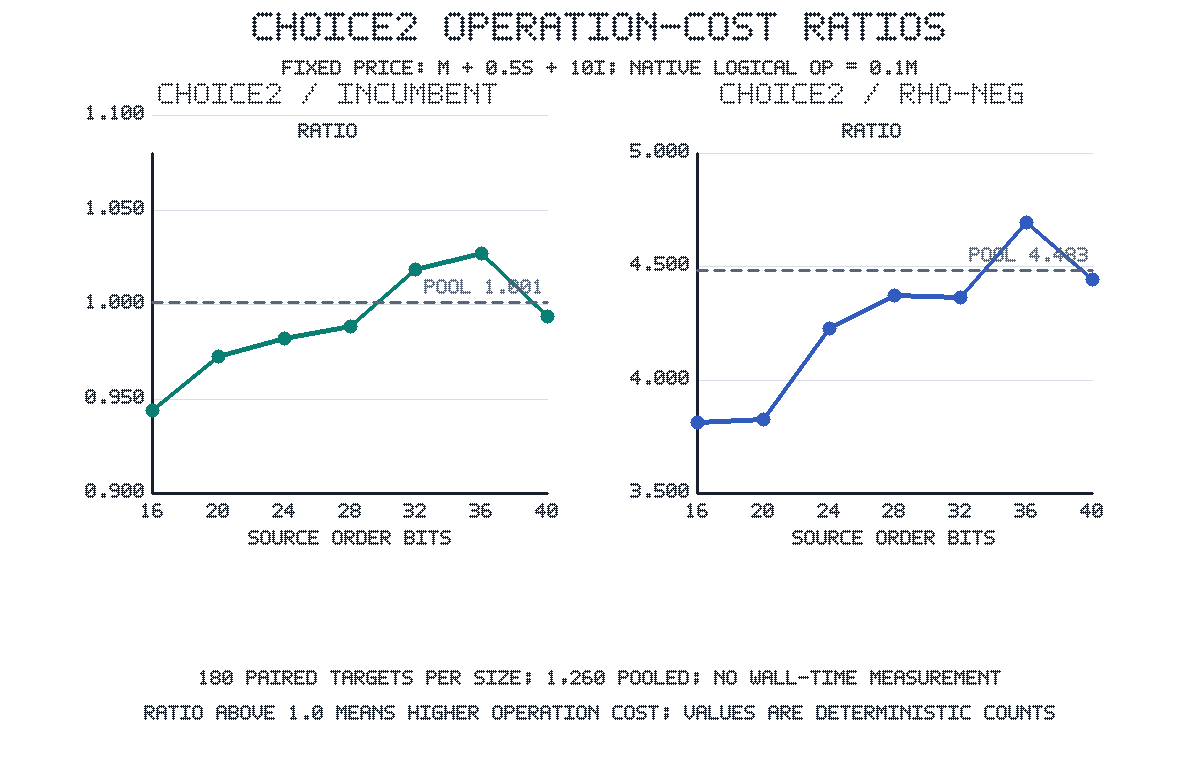
\includegraphics[width=\linewidth]{choice2-operation-cost-ratios.png}
\caption{Deterministic operation-cost ratios at the fixed price above. The dashed line is the pooled sum ratio. No statistical interval is applicable to these fixed counts.}
\end{figure}

At this fixed price, pooled two-choice/incumbent cost is 1.000857; two-choice/source-negation-rho cost is 4.483247. Across the 21 curves, the source report gives a two-choice/incumbent range of 0.933237 to 1.102391, so pooled parity does not establish a consistent per-curve improvement.

\section*{Limits and provenance}
These are operation-count estimates (L0). No isolated wall timing, A/A timing, hardware-speed claim, fastest-external comparison, or end-to-end DLP advantage is established. The result is not entered into performance history or the IC leaderboard. Projective arithmetic and the other four leads remain incomplete as documented in the source report.

Source data (copies beside this report): \texttt{genus2-choice2-price-grid.csv} and \texttt{genus2-choice2-summary.json}. Canonical source paths: \texttt{research/five\_leads\_e2e\_20261019/results/genus2-choice2-price-grid.csv} and \texttt{research/five\_leads\_e2e\_20261019/results/genus2-choice2-summary.json}. Replay receipts: \texttt{results/replay-audit-summary.json} and \texttt{sessions.tar.zst} in \texttt{research/five\_leads\_e2e\_20261019/}. Reproduction command: \texttt{python3 research/five\_leads\_e2e\_20261019/reports/choice2-operation-costs-20261019/render.py} followed by \texttt{tectonic report.tex} from this directory.
\end{document}
